%%=============================================================================
%% Methodologie
%%=============================================================================

\chapter{\IfLanguageName{dutch}{Methodologie}{Methodology}}
\label{ch:methodologie}

%% TODO: Hoe ben je te werk gegaan? Verdeel je onderzoek in grote fasen, en
%% licht in elke fase toe welke stappen je gevolgd hebt. Verantwoord waarom je
%% op deze manier te werk gegaan bent. Je moet kunnen aantonen dat je de best
%% mogelijke manier toegepast hebt om een antwoord te vinden op de
%% onderzoeksvraag. 

In the study two different algorithms will be used to compare quantum computing with classical computing. 
The fact that there are two algorithms and not just one is because a quantum computer can't run a normal algorithm: is has to be updateted to a new form, the quantum algorithm.
This chapter will explain more about the algorithms, which one is chosen and how to rewrite it to a quantum algorithm. Since there will be a look into the complexities of an algorithm, there will be an explanation on what this is.
Both the time and space complexities will be clarified. Running the classical algorith is easy since it can be done on a classical computer. For the quantum algorithm: it has to be run on a quantum computer.
To simulate this the study will be using IBM's Quantum composer, but more information about that in \ref{sec:Composer}.
\section{Algorithms}
Originally there was a survey build for this study from which algorithms that are frequently used in businesses nowadays would come. This survey was spread out to the public across multiple media sources, and on several occasions.
Yet there was not much response on this survey, so the decision to not use this was made. Another algorithm will be used: the algorithm to find factors of large numbers. This was chosen because this is, at the moment writing, this forms the biggest 'threat' from quantum computing to the world.
This is because RSA encryption is based on the fact that factorization of large numbers, like bank numbers or cryptosystems \autocite{Shor}, takes a very long time to do for classical computers. But if a quantum computer could do it in mere seconds or even minutes the entire bankin system could fall, no transaction would be safe anymore.
This algorithm has already been made and is known as Shor's algorithm \autocite{Shor}.
\subsection{Complexities of algorithms}
\label{subsec:Complexities}
There are two complexitites used to describe algorithms: Time and Space. Those complexities describe the efficiency of the algorithm. By doing this there is a general way to compare two algorithms with eachother: calculate the complexitites of both and compare them.
Time complexity is the time needed to run an algorithm as a function of the length of the input \autocite{Timecomp}. The length of the input is the amount of operations that have to be run. Say there is an algorithm with a for-loop from 1 to 100.
In this loop it just adds the numbers up, then the algorithm has to run 100 operations inside the loop and 100 operations to check if the loop is fulfilled. That makes a total of 200 operations just to add the numbers from 1 to 100.
The amount of time needed can also differ from computer to computer: a pc with a better processor, say an Intel Core i7 with a base frequency of 4,9 GHz may have significant better times than a lower quality processor: Intel Core i3 with a base frequency of 2,9 GHz.
To note the time complexity of an algorithm, the big-O notation is used. As read in section 4.2 of \textcite{Hidary_2019}, the big-O notation is used to describe the asymptotic upper bound or the worst case scenario. In the case of time complexity that's the logest time it will take to run the algorithm.
In the space complexity, the memory needed for to run the algorithm is taken into account to calculate the efficiency of the algorithm \autocite{Abhishek2021Ruimte}. As in time complexity, space complexity too uses the big-O notation to note it's worst case scenario. Another notation that could be used is the asymptotic lower bound or the best case scenario: the omega notation.
In this study, only the big-O notation will be handeled when speaking about the complexity of an algorithm.
\subsection{Everything about quantum algorithms}
Eventhough all the classical algorithms can be run on a quantum computer, the superpositions of qubits or entanglement would never be used \autocite{qalgo} and \autocite{quantumalgo} ans thus it would make the quantum computer a very expensive computer.
The term quantum algorithm is only used for an algorithm when it uses features of quantum computing like superposition or entanglement.
Eventhough a quantum computer may be able to solve some of the algorithms faster than a classical computer, it can't help with undecidable problems. If there is no know classical algorithm to solve a problem, there won't be a quantum one \autocite{undecidable} and \autocite{quantumalgo}.
The algorithm used in this study is an algorithm used for factoring very large numbers. The best classical algorithm to do is is known as the general number field sieve \autocite{GNFS}, and its quantum counterpart is known as Shor's algorithm \autocite{Shor}.
Quantum algorithms are often shown in a quantum circuit as can be seen in figure \ref{fig:Quantum circuit}. A quantum circuit has 2 main elemets: the qubits represented by the horizontal lines and the quantum gates or operations represented by the squares on teh lines.
When a qubit line crosses a gate it means that that specific gate is used on that qubit. There are different gates, but those will be explained in \ref{sec:gates}.

\begin{figure} [h]
    \centering
    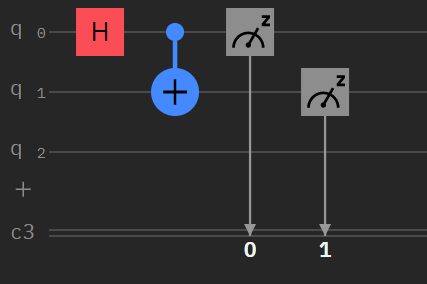
\includegraphics[width=\textwidth]{img/circuitVB.PNG}
        \caption{This is an example of a simple quantum circuit}
        \label{fig:Quantum circuit}
\end{figure}

\section{Quantum composer}
\label{sec:Composer}
Quantum composer is a tool to build quantum circuits. After building the circuits, they can be run on the quantum computer at IBM. This is an easy-to-use beginners tool. The circuits can be made by a drag and drop system.
At the same time that the circuits is being build, the tool converts it into code in OpenQuasm2.0. It also shows the probabilities of each qubit and the blockspehere representation of the qubits.
In figure \ref{fig:Quantum composer} A screenshot of Quantum composer can be see. At the top all the gates can be found and right under the gates the circuits is build. The right part of the screen is the OpenQuasm2.0 code.
The bottom shows the blochsphere-representation and the probabilities.

\begin{figure} [h]
    \centering
    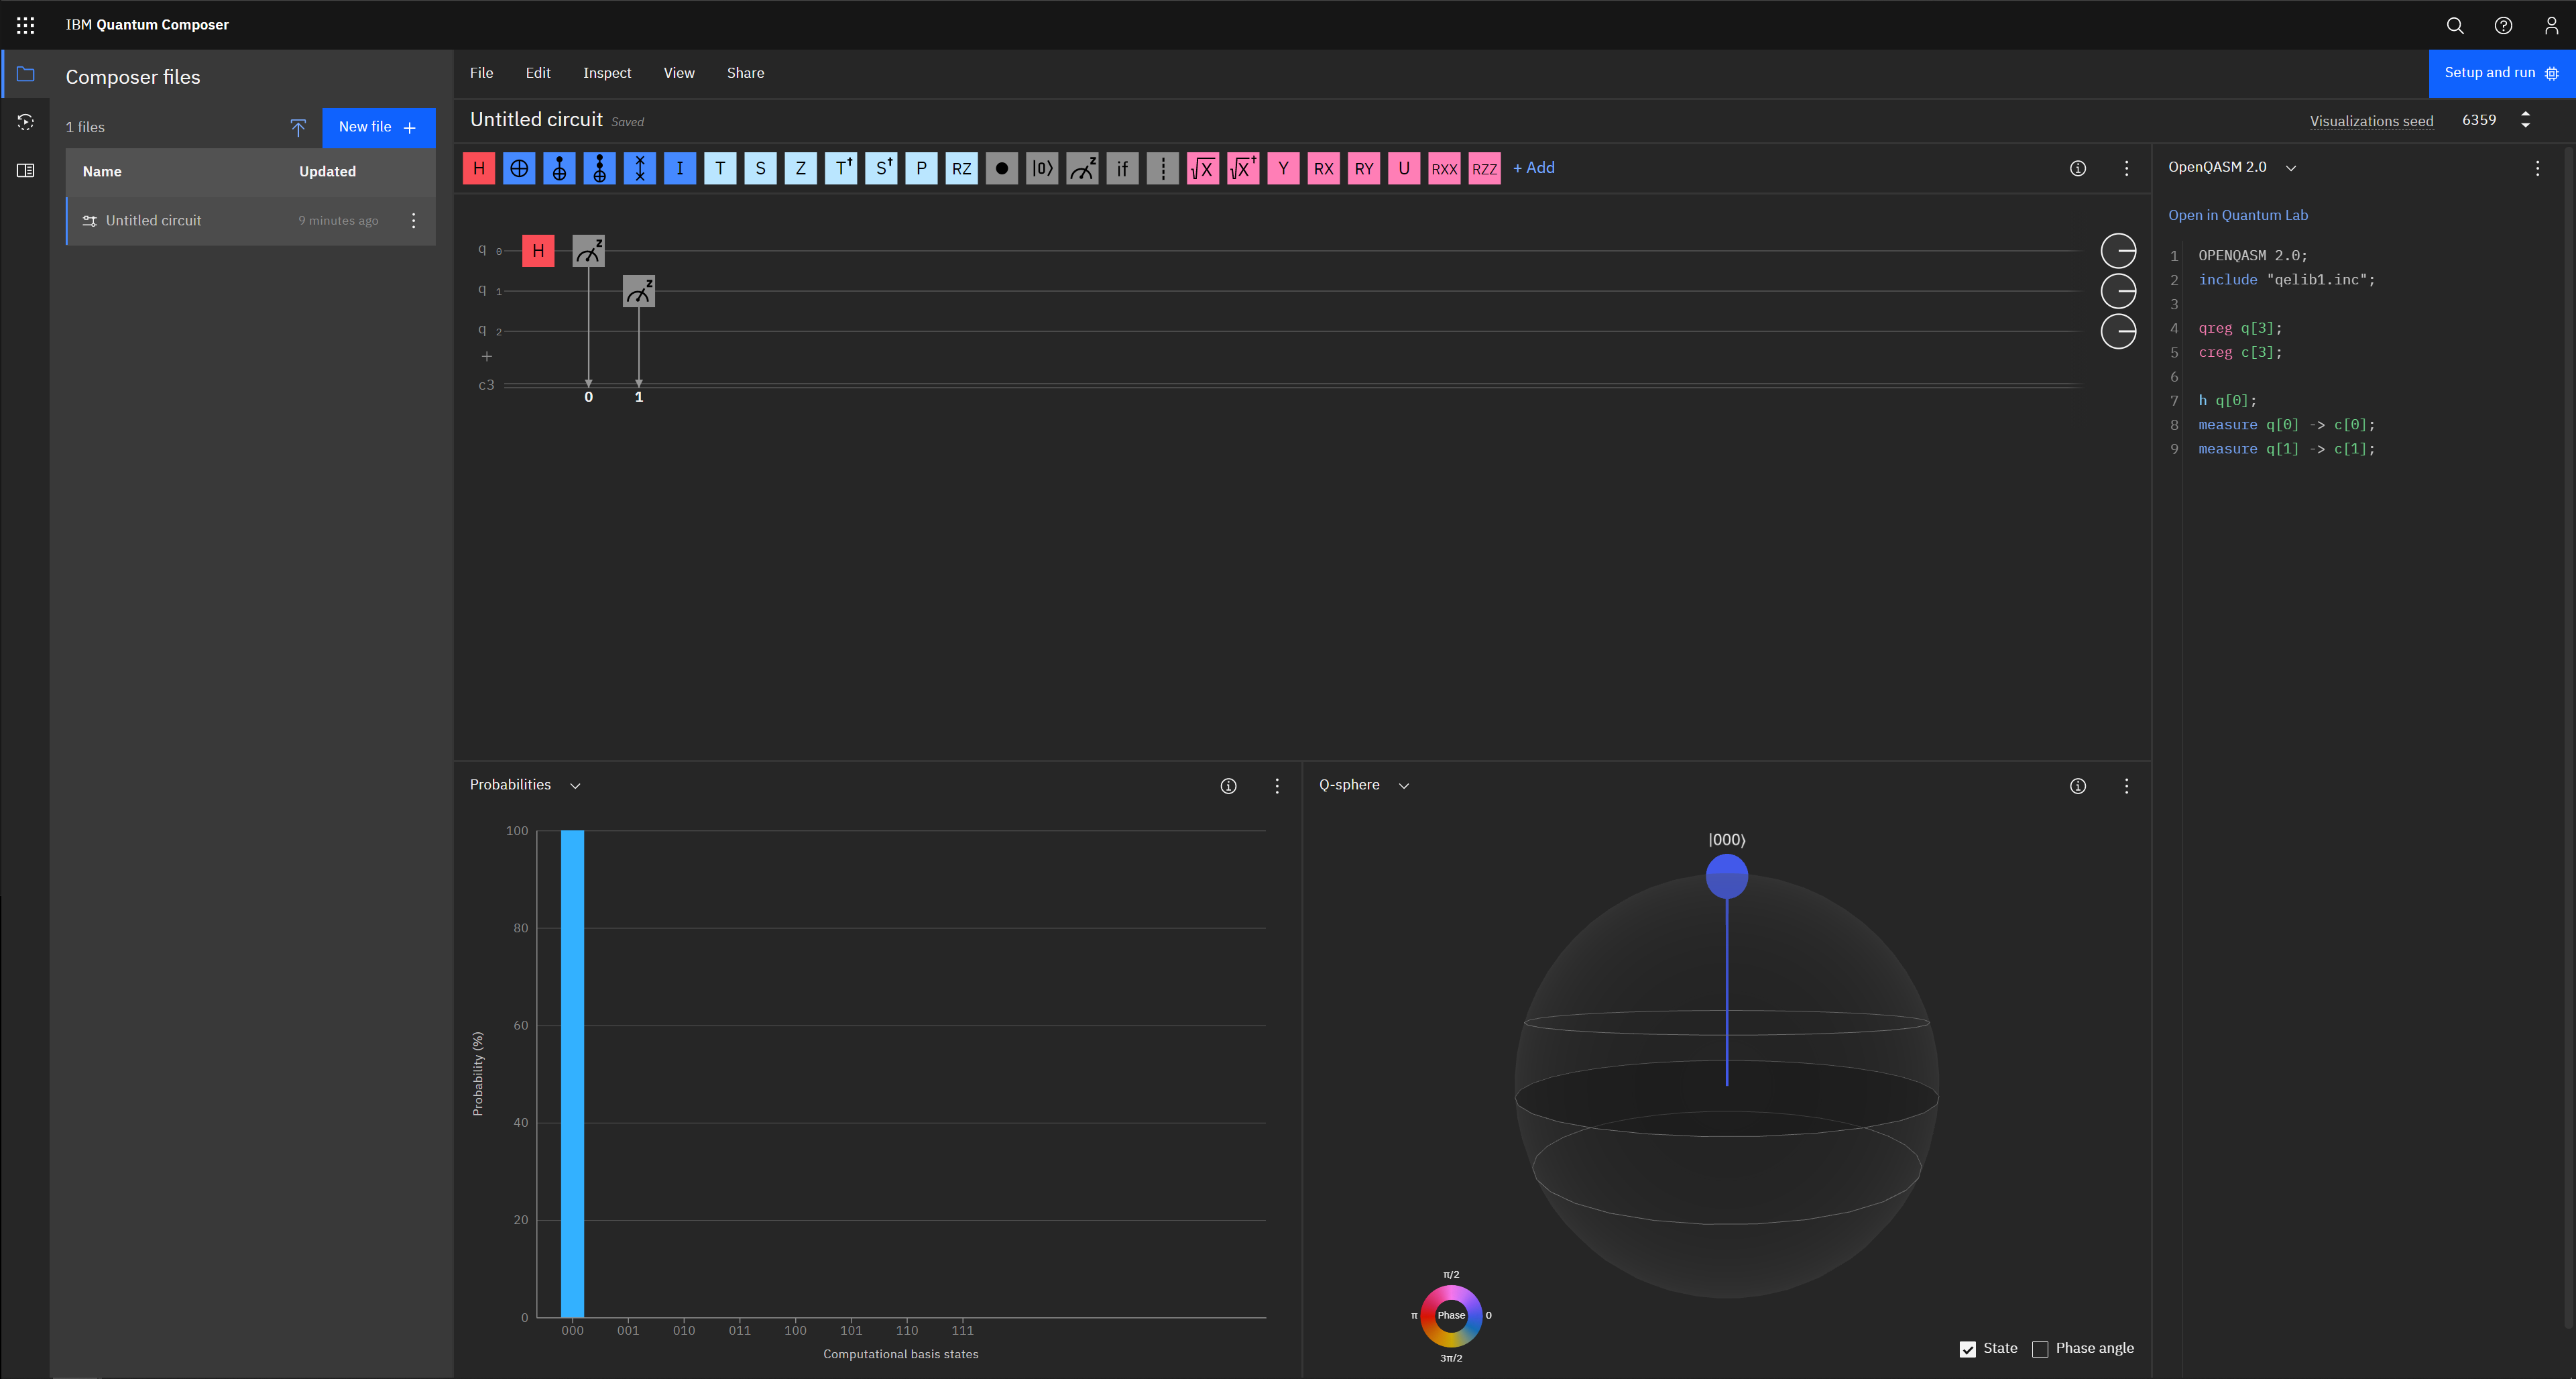
\includegraphics[width=\textwidth]{img/composer.PNG}
        \caption{Screenshot of Quantum composer}
        \label{fig:Quantum composer}
\end{figure}